Our team has one robot, called Judith (see Fig.~\ref{fig:judith}). Judith is a robot based on Peoplebot robot~\cite{peoplebot:2001} and KUKA youBot arm~\cite{youbot:2016}. As shown in Fig.~\ref{fig:judith}, Judith has: 1 Microsoft Kinect for Xbox 360; 2 Sonar Arrays; 2 Infrared Sensors; 1 iPAD 2; 1 Microphone Yoga HT-320A; 1 Touch Sensors Array; 2 Speakers; 1 Emergency Button; and 1 Hokuyo Laser URG-04LX-UG01.

\begin{figure}[ht!]
    \centering
    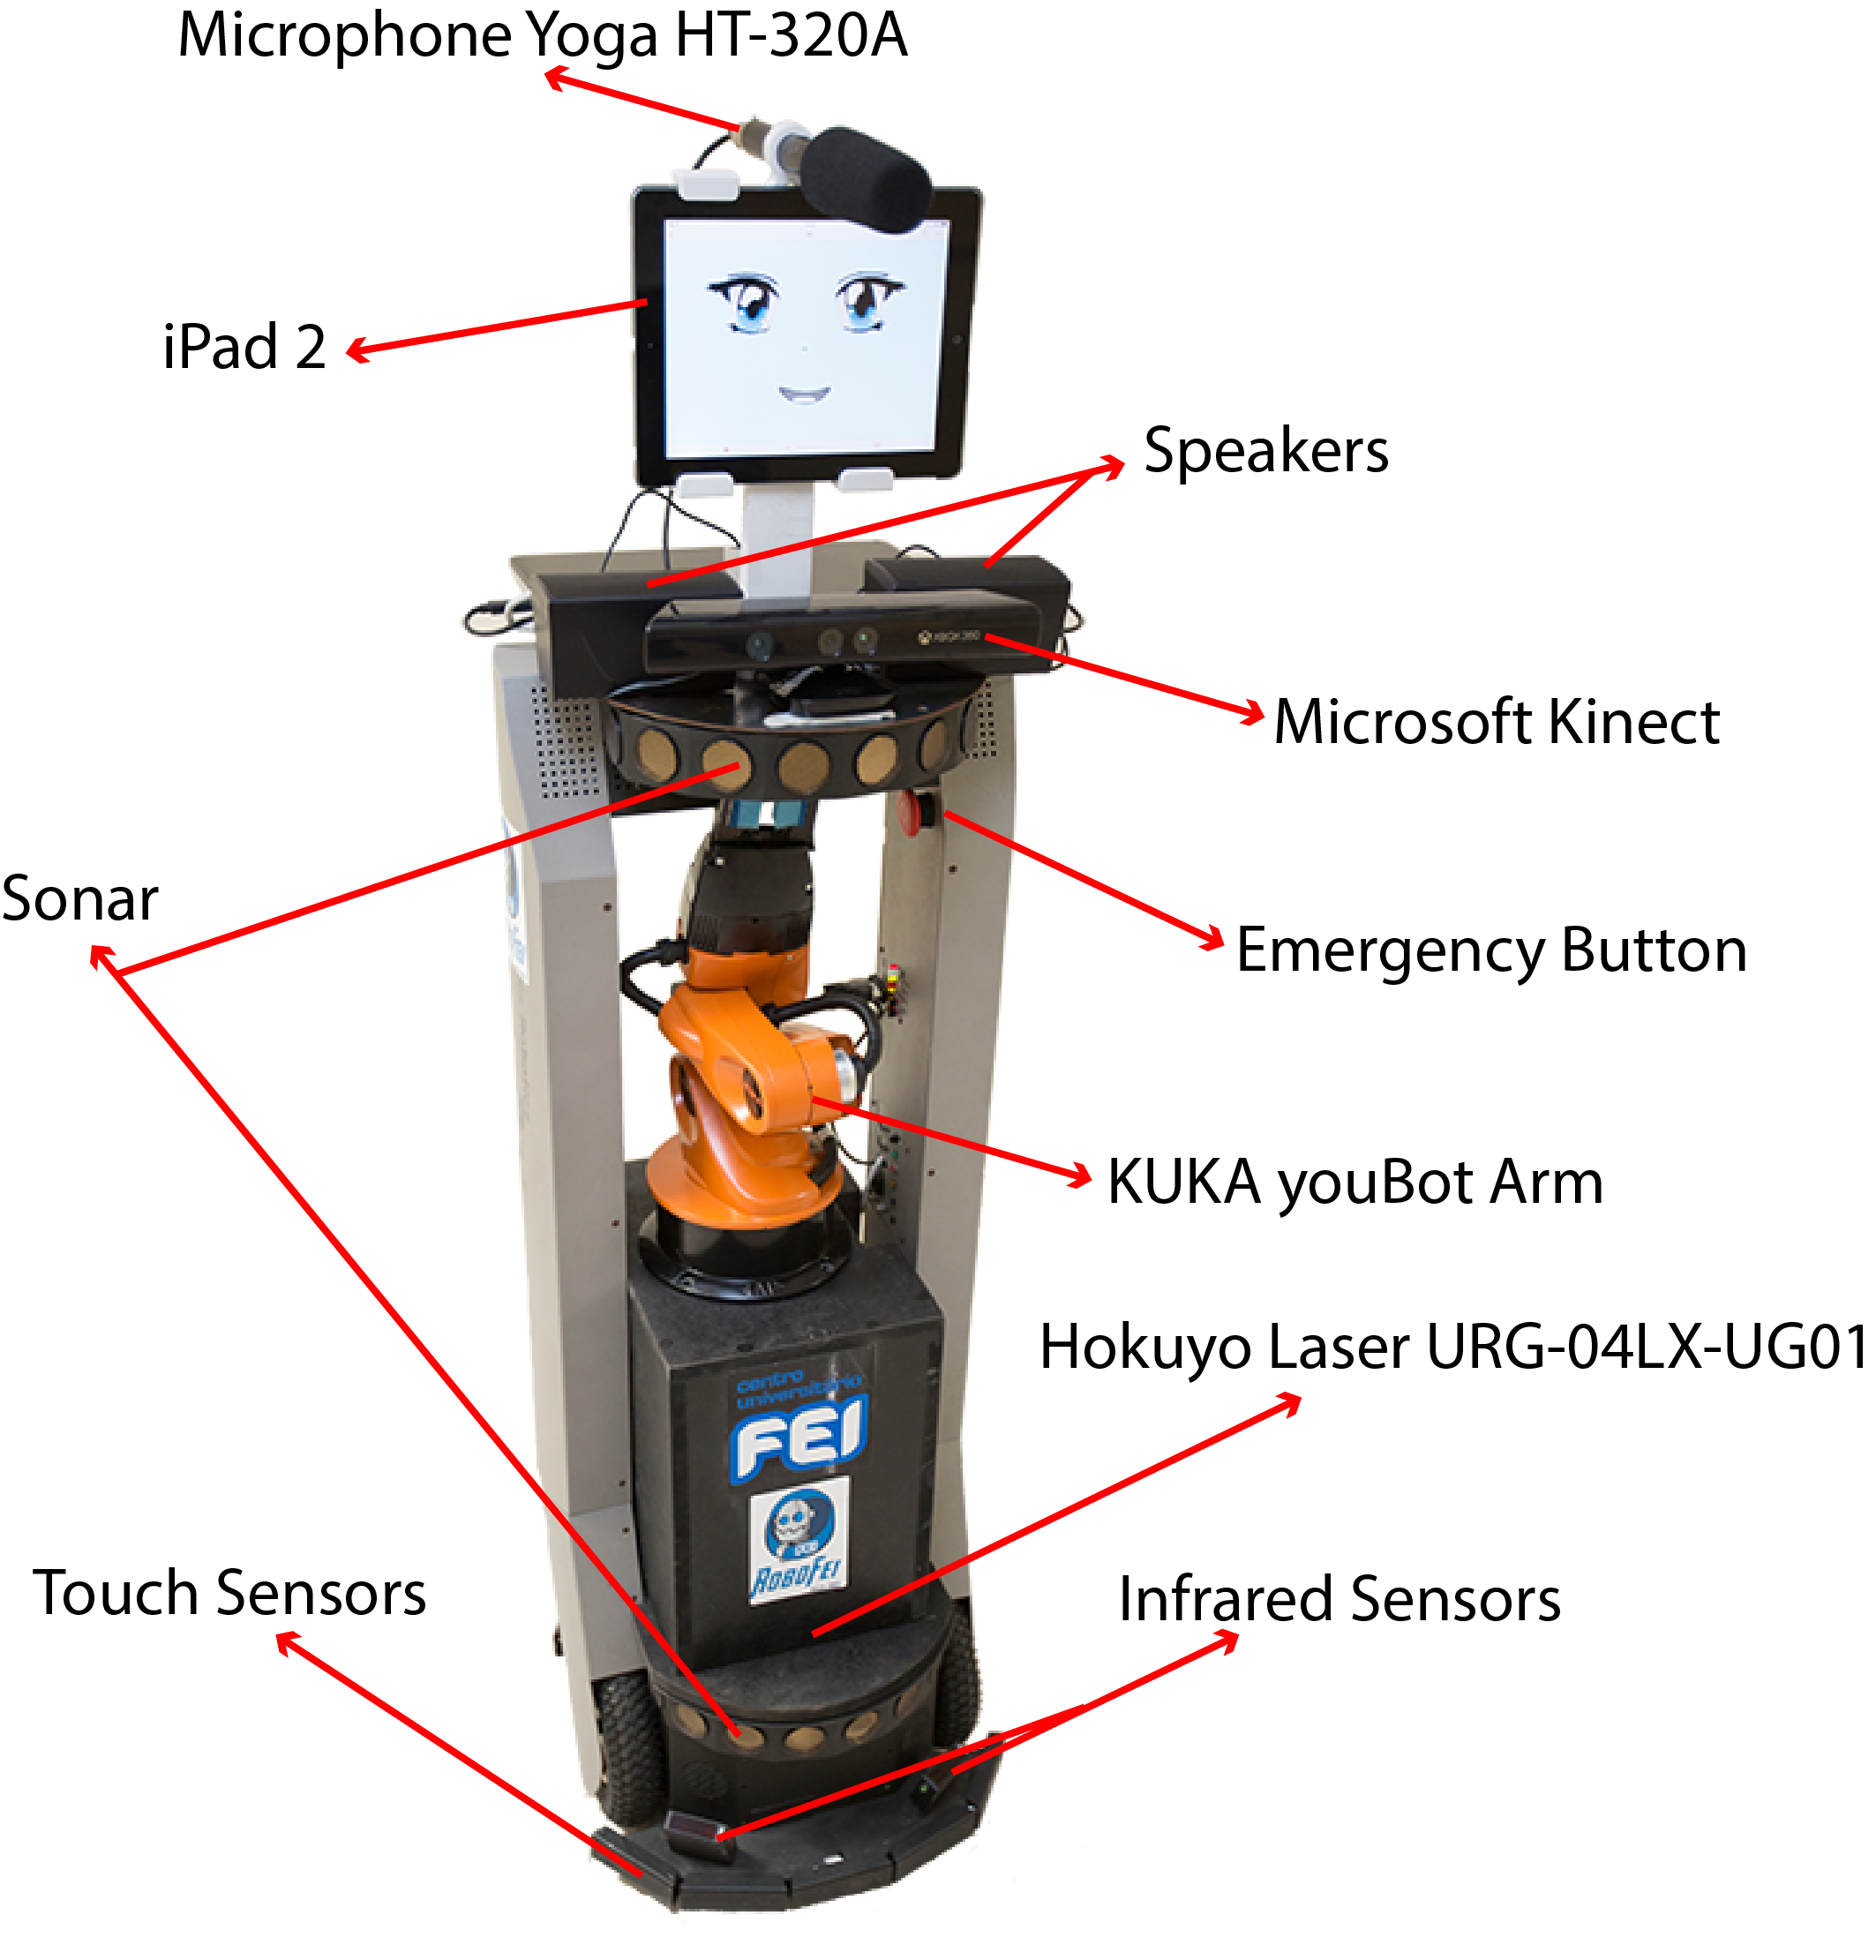
\includegraphics[height = 7.2cm]{figures/judith_info.png}
    \caption{RoboFEI's Judith}
    \label{fig:judith}
\end{figure}

Working with two different ready robots present some challenges. First of all, each one has electric source with different voltage. KUKA youBot arm needs 24v to work while Peoplebot works with 12v. To put Peoplebot and KUKA youBot arm together, we need to build a circuit for connecting both batteries kit together. This circuit is important to keep all parts of robots safe in case of electric damage on overcharge. It also helps to make both robots work at the same time.

Peoplebot has a vertical grip which needs to be removed for attaching KUKA youBot arm. To attach the new arm, we built a support for keeping it on the right height to manipulate objects on the table. KUKA youBot arm weighs 16.53 pounds so we made a wood support to hang up with this weight. With all mechanical and electrical project setup, we need to connect both robots on main computer.

Here we face another problem, because our computer has only USB ports as a device input options or Ethernet and WiFi connections. Peoplebot can interface with a serial port RS232 and KUKA youBot arm interfaces with a real-time EtherCAT. To solve this problem, we use EtherCAT connection for KUKA youBot arm, and for Peoplebot platform needs a RS232 to USB converter for helping interface with computer.

As main computer we have been using an ASUS Ultrabook 14'' Touch-Screen Laptop with Intel Core i5, 4GB Memory, 500GB Hard Drive. It has only 3 USB ports supporting all devices. To enable more ports, we have used a USB hub to increase number of devices interfaced. As iPad need a annual license to develop programs, we are changing for an Android tablet which allow us to develop a interactive face for our robot Judith.

Platform used by Peoplebot turns the transportation very difficult for us. In that way, we have worked on a module platform using 3D printer and aluminum parts. We want to accomplish this project until Robocup 2016 in Germany.